\documentclass[11pt,a4paper]{article}
\usepackage[T1]{fontenc}
\usepackage{lmodern,amsmath,amssymb,amsthm,mathtools}
\usepackage[margin=25mm]{geometry}
\usepackage{microtype,booktabs,array,xcolor,graphicx}
\usepackage{tikz,pgfplots}
\pgfplotsset{compat=1.18}
\definecolor{dirichlet}{RGB}{30,83,150}
\definecolor{neumann}{RGB}{168,55,45}
\definecolor{paperlink}{RGB}{0,0,114}
\usepackage[colorlinks=true,linkcolor=paperlink,citecolor=paperlink,urlcolor=paperlink]{hyperref}
\usepackage{fancyhdr}
\usepackage{placeins}
\hypersetup{pdftitle={Classical Casimir force: BEM implementation and numerical illustrations}}
\pagestyle{fancy}\fancyhf{}
\fancyhead[L]{\small Classical Casimir force: numerical report}
\fancyhead[R]{\small\thepage}
\setlength{\headheight}{14pt}
\setlength{\parindent}{1.25em}\setlength{\parskip}{0pt}
\setlength{\emergencystretch}{1em}
\brokenpenalty=10000
\numberwithin{equation}{section}
\newcommand{\dd}{\,\mathrm d}
\newcommand{\ii}{\mathrm i}
\newcommand{\Rea}{\operatorname{Re}}
\newcommand{\Ima}{\operatorname{Im}}
\newcommand{\norm}[1]{\lVert#1\rVert}
\makeatletter\let\inputrows\@@input\makeatother
\newcommand{\PilotSeconds}{488.3}
\newcommand{\PeakRSS}{0.95}
\newcommand{\BackendVersion}{0.3.1}
\newcommand{\CheckCount}{16}
\newcommand{\SourceDigest}{8d706dca230ad02f}
\newcommand{\ExactD}{7.260312510}
\newcommand{\ExactN}{1.487792351}

\title{Classical Casimir force:\\BEM implementation and numerical illustrations}
\author{Arne Hofmann}\date{4 November 2026}
\begin{document}
\maketitle
\begin{abstract}
A boundary element implementation computes the force on each component of a collection of obstacles illuminated by a plane wave. It uses combined-field equations for Dirichlet and Neumann scattering, followed by boundary-traction integration. Independent checks use analytic sphere scattering, far-field momentum balance, and a position derivative of the scattering amplitude. The local pilot exhibits decreasing sphere errors and decreasing discrepancies between the two force calculations. This report gives the force conventions and implementation, expresses benchmark measurements in terms of mesh size, and presents a fixed-resolution distance curve for two Dirichlet spheres. The measurements are numerical illustrations for scattering theory; the benchmark checks do not imply a uniform error bound for the distance curve.
\end{abstract}

\section{What has been computed}
The local pilot uses unit sphere radius, unit incident amplitude, and wavenumber~$k=1$, with three inscribed icosahedral refinements. Two-sphere checks use surface gap~$g=2$, transverse illumination, and two mesh levels. Additional checks test amplitude scaling, translation and rotation, reflection symmetry, and scattering near interior eigenfrequencies. All~\CheckCount{} programmed pilot checks passed in \PilotSeconds{} seconds, with peak observed process-tree resident memory of \PeakRSS{}~GiB. These are finite numerical checks, not certified error estimates.

The pilot ran with Bempp-cl~\BackendVersion{}, NumPy~1.26.4, SciPy~1.14.1, and Numba~0.60.0. The historical environment is recorded in \texttt{requirements-local.lock}. The distance curve uses Bempp-cl~0.3.2, NumPy~2.1.3, SciPy~1.15.2, and Numba~0.61.0; its full version record accompanies the data.

Narrow convergence checks guide a mesh choice for scattering-theory illustrations, with force errors around one percent in the benchmark cases. This report does not claim uniform accuracy over a separation interval. The distance curve contains 150 computed samples at a fixed mesh and quadrature order.

\section{Force conventions}
Let~$\mathcal O$ be a union of disjoint bounded obstacles, and let~$\nu$ point from each obstacle into the exterior. The incident field and far-field convention are
\begin{equation}\label{eq:field}
 u^{\rm inc}(x)=A\mathrm e^{\ii k d\cdot x},\qquad
 u^{\rm sc}(r\theta)=\frac{\mathrm e^{\ii kr}}r f(\theta;d)+O(r^{-2})\,,
\end{equation}
where~$d$ and~$\theta$ are unit vectors and~$k>0$. The amplitude~$A$ is included in~$f$. The unpolarized Helmholtz stress tensor and component force are
\begin{align}
 T_{ij}[u]&=\Rea(\partial_i u\,\overline{\partial_j u})
       -\tfrac12\delta_{ij}(|\nabla u|^2-k^2|u|^2)\,,\label{eq:stress}\\
 \mathbf F_b&=-\int_{\partial\mathcal O_b}T[u]\nu\dd S\,.\label{eq:force}
\end{align}
Differentiation of~\eqref{eq:stress} gives
\begin{equation}
 \partial_jT_{ij}[u]=\Rea\bigl((\Delta\bar u+k^2\bar u)\partial_i u\bigr)\,.
\end{equation}
Thus stress flux is conserved in an obstacle-free Helmholtz region. This fixes the sign of the force: a nonabsorbing isolated sphere in a travelling plane wave has force in direction~$d$.

Write~$\phi=u|_{\partial\mathcal O}$ and~$q=\partial_\nu u|_{\partial\mathcal O}$. The boundary conditions simplify~\eqref{eq:force} to
\begin{align}
 \mathbf F_b^{D}&=-\tfrac12\int_{\partial\mathcal O_b}|q|^2\nu\dd S\,,\label{eq:dirichlet}\\
 \mathbf F_b^{N}&=\tfrac12\int_{\partial\mathcal O_b}
       (|\nabla_\Gamma\phi|^2-k^2|\phi|^2)\nu\dd S\,.\label{eq:neumann}
\end{align}
For Dirichlet conditions the tangential gradient vanishes; for Neumann conditions the normal derivative vanishes. The implementation integrates these two expressions directly.

If~$u$ is a pressure phasor in pascals with time convention~$p(x,t)=\Rea(u(x)\mathrm e^{-\ii ck t})$, the time-averaged acoustic momentum tensor is~$T[u]/(2\rho c^2k^2)$. This follows by inserting~$v=\nabla u/(\ii\rho ck)$ into
\begin{equation}
 \Pi=\left(\frac{|u|^2}{4\rho c^2}-\frac{\rho|v|^2}{4}\right)I
       +\frac\rho2\Rea(v\otimes\bar v)\,.
\end{equation}
With mesh lengths in metres, multiply~\eqref{eq:force} by~$1/(2\rho c^2k^2)$ to obtain newtons. This conversion assumes that the computed field is pressure; it must not be reused unchanged for a velocity-potential normalization.

For equal spheres centered on the~$x$-axis, set~$e=(1,0,0)$ and define
\begin{equation}\label{eq:separation}
 F_{\rm sep}=\tfrac12(\mathbf F_2-\mathbf F_1)\cdot e\,.
\end{equation}
The corresponding displacement moves the centers by~$\pm\tfrac12 e\dd g$, so their work is~$F_{\rm sep}\dd g$. Positive~$F_{\rm sep}$ means repulsion. The total force~$\mathbf F_1+\mathbf F_2$ is reported separately. The driven field can carry momentum away, so individual forces need not be equal and opposite. Interaction forces subtract an isolated-obstacle calculation with the same incident wave, location and mesh.

\section{Boundary integral implementation}
With outgoing Green function~$G_k(x,y)=\mathrm e^{\ii k|x-y|}/(4\pi|x-y|)$, denote single and double layer potentials by~$S$ and~$D$. Bempp's boundary operators are~$V$, $K$, $K'$ and~$W=-\gamma_1D$; this last sign is material~\cite{bempp-operators}. Green's exterior representation and its two traces give
\begin{align}
 u&=u^{\rm inc}+D\phi-Sq\,,\\
 (\tfrac12 I-K)\phi+Vq&=\phi^{\rm inc}\,,\label{eq:trace0}\\
 W\phi+(\tfrac12 I+K')q&=q^{\rm inc}\,.\label{eq:trace1}
\end{align}
The incident traces are~$\phi^{\rm inc}=u^{\rm inc}$ and~$q^{\rm inc}=\ii k(d\cdot\nu)u^{\rm inc}$.

For the Dirichlet problem, combine~\eqref{eq:trace0} and~\eqref{eq:trace1} to solve
\begin{equation}\label{eq:cfieD}
 (\tfrac12I+K'-\ii kV)q=q^{\rm inc}-\ii k\phi^{\rm inc}\,,
 \qquad u^{\rm sc}=-Sq\,.
\end{equation}
For the Neumann problem, the chosen combined equation is
\begin{equation}\label{eq:cfieN}
 (\tfrac12I-K+\ii W/k)\phi=\phi^{\rm inc}+\ii q^{\rm inc}/k\,,
 \qquad u^{\rm sc}=D\phi\,.
\end{equation}
These coupled traces replace an unprotected single-layer inversion at real interior eigenvalues. The implementation uses piecewise constant~$q$ for~\eqref{eq:cfieD} and continuous piecewise linear~$\phi$ for~\eqref{eq:cfieN}. Operators are assembled in double precision with the CPU/Numba backend. GMRES uses the Galerkin mass matrix as a left preconditioner, with relative residual tolerance~$10^{-9}$.

The Dirichlet traction integral is exact for a constant discrete~$q$ on each flat triangle. For a triangle of area~$B$, the Neumann surface gradient is constant, and the remaining mass integral is evaluated as
\begin{equation}
 \int_\triangle|\phi_h|^2\dd S
  =\frac B{12}\left(\sum_{j=1}^3|\phi_j|^2+
                         \left|\sum_{j=1}^3\phi_j\right|^2\right)\,.
\end{equation}
Exact integration of a discrete trace does not remove trace error or the geometry error of the polygonal surface. Spatial refinement and independent force comparisons are therefore essential.

Sphere meshes are generated by radial projection of subdivided icosahedra. The solver also accepts imported closed triangular component meshes. It checks edge closure, orientation, nondegenerate elements, connectivity of each component label, and absence of shared vertices between components. General surface self-intersection, inter-component collision, and nested-obstacle geometry are not automatically certified; imported geometry must satisfy the exterior-scattering assumptions.

For a sphere of radius~$a$, the mesh size is the maximum Euclidean triangle diameter,
\begin{equation}\label{eq:mesh-size}
 h=\max_{T\in\mathcal T_h}\operatorname{diam}(T)
   =\max_{[v_i,v_j]\text{ a mesh edge}}|v_i-v_j|\,.
\end{equation}
We report the dimensionless ratio~$h/a$. The values are measured from the actual triangulations, not estimated from the triangle count. The command-line option~\texttt{--mesh-size} specifies an upper bound on~$h/a$ and selects the coarsest member of this nested mesh family that satisfies it. For example, \texttt{--mesh-size 0.2} selects~$h/a\simeq0.164647$, with 1280 triangles per sphere. The requested bound and the attained size are both recorded. The refinement-level selector remains available as~\texttt{--mesh-level}.

\section{Independent force calculations}
\subsection{Momentum balance}
The far-field momentum flux of~\eqref{eq:field} gives the total Helmholtz force
\begin{equation}\label{eq:momentum}
 \mathbf F_{\rm tot}=4\pi k\Ima(\bar A f(d;d))d
    -k^2\int_{\mathbb S^2}\theta|f(\theta;d)|^2\dd\theta\,.
\end{equation}
The first term is the incident--scattered interference contribution. For a nonabsorbing exact solution, the optical theorem reads
\begin{equation}\label{eq:optical}
 \frac{4\pi}k\Ima(\bar A f(d;d))
    =\int_{\mathbb S^2}|f(\theta;d)|^2\dd\theta\,.
\end{equation}
Both sides of~\eqref{eq:optical} are recorded rather than enforcing their equality on the approximate solution. Angular integration uses Gauss--Legendre quadrature in~$\cos\theta$ and a periodic trapezoidal rule in azimuth. Increasing the angular order independently checks this integration.

\subsection{Position derivative}
Translate component~$b$ by~$s e_j$, holding the global incident wave and outgoing directions fixed. The force is
\begin{equation}\label{eq:position}
 F_{b,j}=2\pi\Rea\bigl(\bar A\,\partial_s f(d;d)\bigr)
    +k\Ima\int_{\mathbb S^2}\overline{f(\theta;d)}\,
                              \partial_s f(\theta;d)\dd\theta\,.
\end{equation}
Here the derivative moves just the selected component. Centered differences at~$\delta$ and~$\delta/2$ use identical mesh connectivity translated rigidly, avoiding remeshing noise. The pilot uses~$\delta=0.02a$; this displacement step is distinct from the mesh size~$h$.

The constants in~\eqref{eq:position} can be checked from the scattering operator. For unit incident amplitude its kernel, in propagation-direction coordinates, is~$S=I+\ii kf/(2\pi)$. Set~$P=-\ii S^*\partial_sS$. The incoming/outgoing flux identity gives~$F_{b,j}=4\pi^2|A|^2P(d,d)/k$. To see the normalization, use the three-dimensional Herglotz-wave normalization~$k(2\pi)^{-1}\int\mathrm e^{-\ii k\omega\cdot x}\Phi(\omega)\dd\omega$; the incident direction~$d$ corresponds to~$\omega=-d$. Expanding the smooth kernel of~$P$ then gives~\eqref{eq:position}. No squared~$L^2$ norm is assigned to the delta distribution defining a plane-wave channel.

The flux-to-stress step also fixes the sign. For a boundary displacement~$v=Y\cdot\nu$, differentiating the Dirichlet condition gives~$\dot u=-vq$ and hence boundary flux~$\int v|q|^2$. Differentiating the Neumann condition gives~$\partial_\nu\dot u=\operatorname{div}_\Gamma(v\nabla_\Gamma u)+k^2vu$ and boundary flux~$-\int v(|\nabla_\Gamma u|^2-k^2|u|^2)$. In either case~\eqref{eq:dirichlet}--\eqref{eq:neumann} equal minus one half of that flux. This recovers~$kP$ in this generalized-eigenfunction normalization.

As a second normalization check, translating the whole configuration changes the far field by~$f_s(\theta;d)=\mathrm e^{\ii ks(d-\theta)\cdot e_j}f_0(\theta;d)$. Substitution into~\eqref{eq:position}, followed by~\eqref{eq:optical}, gives~\eqref{eq:momentum} componentwise.

\subsection{Analytic sphere}
For a sphere of radius~$a$ centered at the origin, expand the incident plane wave into partial waves. Enforcing the boundary condition in each angular momentum gives
\begin{equation}
 t_\ell^D=-\frac{j_\ell(ka)}{h_\ell^{(1)}(ka)}\,,\qquad
 t_\ell^N=-\frac{j_\ell'(ka)}{h_\ell^{(1)\prime}(ka)}\,.
\end{equation}
The far field and scattered field are
\begin{align}
 f(\theta;d)&=-\frac{\ii A}k\sum_{\ell\ge0}(2\ell+1)t_\ell
                         P_\ell(\theta\cdot d)\,,\\
 u^{\rm sc}(rn)&=A\sum_{\ell\ge0}(2\ell+1)\ii^\ell t_\ell
                       h_\ell^{(1)}(kr)P_\ell(n\cdot d)\,.
\end{align}
Differentiating the same expansion at~$r=a$ supplies the smooth boundary traces for an independent evaluation of~\eqref{eq:dirichlet} or~\eqref{eq:neumann}. This reference uses neither BEM data nor fitted outgoing coefficients. The default truncation is~$\lceil ka+4(ka)^{1/3}+12\rceil$; tests also compare higher cutoffs. At~$k=a=A=1$, the resulting forces in direction~$d$ are~\ExactD{} for Dirichlet and~\ExactN{} for Neumann.

\section{Measured pilot results}
Table~\ref{tab:sphere} separates force, far-field, and near-field errors. The field errors are relative Euclidean sample norms; the force error compares full vectors. Near-field points lie outside the sphere. Figure~\ref{fig:sphere} displays the force errors only: all three measured errors decrease under spatial refinement, despite algebraic residuals already being small on the coarsest meshes.

\begin{table}[htbp]
\centering
\small
\begin{tabular}{crrrrrr}
\toprule
BC & $h/a$ & Triangles & Force along $d$ & Force error (\%) & Far field (\%) & Near field (\%)\\
\midrule
\inputrows{data/sphere-table.tex}
\bottomrule
\end{tabular}
\caption{Unit smooth sphere benchmark at~$k=1$, $A=1$. The meshes are inscribed polygonal approximations; mesh sizes are rounded to six decimals. D and N denote Dirichlet and Neumann.}\label{tab:sphere}
\end{table}

\begin{figure}[htbp]
\centering
\begin{tikzpicture}
\begin{axis}[width=.85\textwidth,height=5.8cm,xmode=log,ymode=log,
 xlabel={mesh size $h/a$},ylabel={relative force error},
 xtick={.164647160064,.324919696233,.618033988750},xticklabels={0.165,0.325,0.618},grid=major,
 legend style={at={(.02,.98)},anchor=north west,font=\small}]
\addplot[dirichlet,thick,mark=*] table[x=h_over_a,y=error,col sep=comma]{data/sphere-dirichlet.csv};
\addlegendentry{Dirichlet}
\addplot[neumann,thick,dashed,mark=square*] table[x=h_over_a,y=error,col sep=comma]{data/sphere-neumann.csv};
\addlegendentry{Neumann}
\addplot[black!60,densely dotted,domain=.15:.65] {0.01};
\addlegendentry{1\% target}
\end{axis}
\end{tikzpicture}
\caption{Relative traction errors~$\norm{\mathbf F_{\rm mesh}-\mathbf F_{\rm exact}}_2/\norm{\mathbf F_{\rm exact}}_2$ against the analytic smooth-sphere reference, plotted against~$h/a$. Lines join three computed values; no convergence order or error bound is asserted. The dotted line marks the practical one-percent target.}\label{fig:sphere}
\end{figure}

At~$h/a\simeq0.164647$, the measured force errors are~$0.810\%$ for Dirichlet and~$1.075\%$ for Neumann. Thus the Dirichlet benchmark is below one percent; the Neumann benchmark is slightly above it. No finer Neumann measurement is claimed here. These checks guide a mesh choice for illustrations rather than a uniform-error certification of a complete force curve.

The two-sphere pilot is repulsive at the tested gap~$g=2a$ for both boundary conditions. Table~\ref{tab:pair} compares the right sphere's separation-direction traction and position-derivative force. The finite-difference step variation is smaller than their discrepancy. That discrepancy decreases on the finer mesh, as does the discrepancy between total traction and momentum force; Figure~\ref{fig:identity} shows the first comparison. This evidence supports the conventions and implementation while retaining visible discretization error.

\begin{table}[htbp]
\centering
\small
\setlength{\tabcolsep}{4pt}
\begin{tabular}{crrrrrr}
\toprule
BC & $h/a$ & Triangles/sphere & $F_{2,x}$ (stress) & $F_{2,x}$ (position) & Difference & Step change\\
\midrule
\inputrows{data/pair-table.tex}
\bottomrule
\end{tabular}
\caption{Equal unit spheres, $k=1$, $g=2$, $d=(0,1,0)$, $A=1$. Position values use~$\delta/2=0.01$; the last column compares centered differences at~$\delta$ and~$\delta/2$. Mesh sizes are rounded to six decimals. All values are Helmholtz forces.}\label{tab:pair}
\end{table}

\begin{figure}[htbp]
\centering
\begin{tikzpicture}
\begin{axis}[width=.85\textwidth,height=5.6cm,xmode=log,ymode=log,
 xlabel={mesh size $h/a$},ylabel={relative force-identity discrepancy},
 xtick={.164647160064,.324919696233},xticklabels={0.165,0.325},grid=major,
 legend style={at={(.02,.98)},anchor=north west,font=\small}]
\addplot[dirichlet,thick,mark=*] table[x=h_over_a,y=error,col sep=comma]{data/identity-dirichlet.csv};
\addlegendentry{Dirichlet}
\addplot[neumann,thick,dashed,mark=square*] table[x=h_over_a,y=error,col sep=comma]{data/identity-neumann.csv};
\addlegendentry{Neumann}
\end{axis}
\end{tikzpicture}
\caption{The componentwise discrepancy~$|F_{2,x}^{\rm stress}-F_{2,x}^{\rm position}|/|F_{2,x}^{\rm position}|$ in Table~\ref{tab:pair}. This is a finite-refinement consistency check at one separation, not a force-error certificate.}\label{fig:identity}
\end{figure}

\FloatBarrier
Assembly quadrature is varied independently from orders~4 to~6 on the finer pair meshes. Rotation, translation and amplitude-squared scaling are checked numerically. Resonance smoke tests use~$k=\pi$ for Dirichlet and~$k\simeq2.081576$ for Neumann; their coarse-mesh field errors are retained in the machine-readable record. These tests demonstrate that the combined formulation remains usable at those examples, not uniform accuracy at every resonance.

\section{Separation-force illustration}
The two unit spheres have Dirichlet boundary conditions, with~$k=A=1$ and transverse incident direction~$d=(0,1,0)$. Figure~\ref{fig:distance} shows~\eqref{eq:separation} at 150 equally spaced surface gaps from~$g/a=0.1$ to~$20$. Every sample uses~$h/a\simeq0.164647$ and regular/singular quadrature orders~6/6. All original case configurations and stored array/mesh hashes were checked before exporting the scientific data.

\begin{figure}[htbp]
\centering
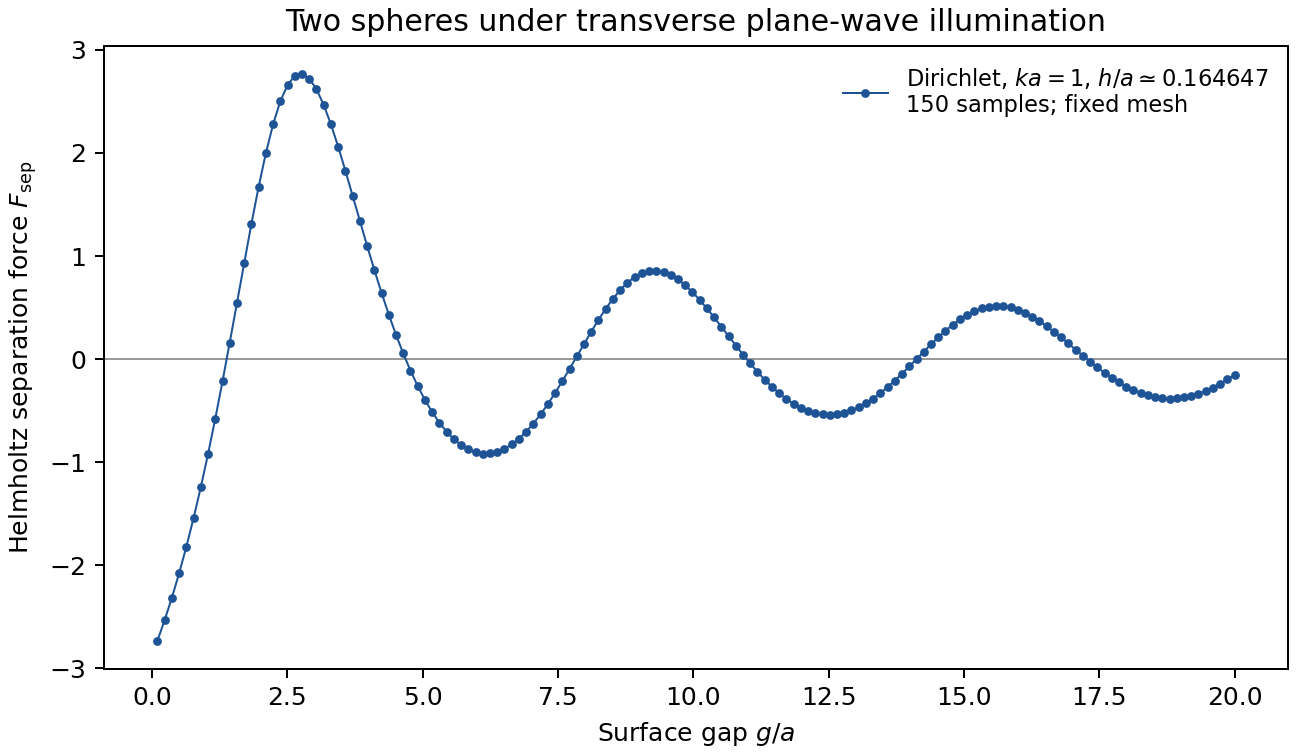
\includegraphics[width=.96\textwidth]{../examples/dirichlet-ka1/force.png}
\caption{Computed Dirichlet separation force for two equal spheres. Positive values indicate repulsion. Lines join adjacent samples; they do not represent a fitted decay law or a convergence band. The curve illustrates oscillation and attenuation at this fixed resolution.}\label{fig:distance}
\end{figure}
\FloatBarrier
The sample values, both component force vectors, mesh and quadrature parameters, software versions and source hashes are supplied in \texttt{examples/dirichlet-ka1}. No isolated-reference subtraction is applied to this force curve. Its accuracy has not been checked uniformly in separation. The narrow sphere and two-sphere pilot checks above provide the available evidence for choosing the mesh.

\section{Reproduction}
The repository contains the local pilot record in \texttt{examples/pilot} and the distance data in \texttt{examples/dirichlet-ka1}. Running \texttt{python scripts/check\_examples.py} checks the scientific exports and numerical-kernel hashes. Running \texttt{python scripts/report\_data.py} regenerates the pilot tables and plot data; \texttt{python scripts/plot\_examples.py} regenerates the distance figure. These commands use the supplied data without rerunning the BEM calculations. Compile this document from its own directory with \texttt{latexmk -pdf numerical-study.tex}.

A small computation is configured in \texttt{configs/example.yaml}. Local commands~\texttt{case}, \texttt{campaign}, and~\texttt{validate} use a process-group watchdog with at most 1200 seconds per campaign and an 8~GiB resident-memory limit. Each completed case records its configuration, software and source versions, force vectors, solver diagnostics and artifact hashes. Resumption verifies these records. Collection reports missing or invalid cases explicitly.

An optional LUIS workflow stages source and all new output below BIGWORK, reuses an existing environment read-only, and runs a compute-node smoke test before the selected distance curve~\cite{luis}. Its configuration and operational instructions are separate from the local solver interface.

\begin{thebibliography}{9}
\raggedright
\bibitem{bempp-operators} The Bempp Team, \emph{The Bempp Handbook: Boundary Operators}, definitions of~$V,K,K',W$ and Galerkin weak forms. \url{https://bempp.com/handbook/api/boundary_operators.html}. Accessed 25 October 2026.
\bibitem{bempp-source} The Bempp Team, \emph{Bempp-cl source and package metadata}, version~0.3.2. \url{https://github.com/bempp/bempp-cl/tree/v0.3.2}. Accessed 25 October 2026.
\bibitem{luis} LUIS, Leibniz Universit\"at Hannover, \emph{Slurm usage guide}. \url{https://docs.cluster.uni-hannover.de/doku.php/guide/slurm_usage_guide}. Accessed 25 October 2026.
\end{thebibliography}
\end{document}
